
\section{Experiment and demonstration}
\label{sec:live}

\begin{figure}
  \centering
  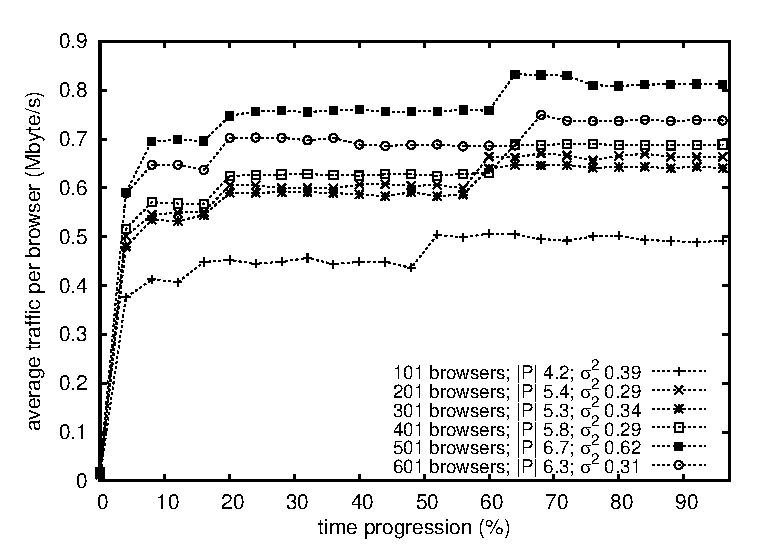
\includegraphics[width=0.49\textwidth]{img/traffic.eps}
  \caption{\label{fig:traffic}Average traffic per second.}
\end{figure}

In laboratory, we tested \CRATE on the Grid'5000 testbed with configurations
involving up till 600 browsers. Figure~\ref{fig:traffic} shows the traffic
generated at each member by intensive editing sessions. Overall, the artificial
authors insert 100 characters per second during 7 hours. The documents reach
millions of characters. Figure~\ref{fig:traffic} shows the combined effects of
\SPRAY and \LSEQ. Indeed, we observe that the traffic logarithmically scales to
the editing session size thanks to \SPRAY. The members of the smallest editing
session (101 browsers) are less traffic intensive than ones of the largest group
(601 browsers).  But the messages transiting the network are important too. The
growth of each plot corresponds to the identifiers size generated by
\LSEQ. Since the document size grows, the identifiers grow, but their growth
slows over insertions.

We would like to confirm the results of the experimentation by performing a live
demonstration of \CRATE that any WWW2016 participant can join. We will start an
\emph{exquisite
  corpse}\footnote{\url{https://en.wikipedia.org/wiki/Exquisite_corpse}}
collaborative storytelling. In this game, we will invite every participant to
continue or update the story initiated by previous participants.

In that regard, we will bootstrap an initial document in our local browser and
share it through a public URL advertised on Twitter. Every participant will be
able to join the session by just clicking on this link. Next, she will freely
add a sentence. During the editing session, we will invite participants to share
and advertise the document with their friends in order to get as many
participants as possible.

During the experiment, we will be able to monitor the evolution of the document
and network. We expect the space complexity of the identifiers associated to
each character to be upper-bounded by $\log(d)^2$ where $d$ is the number of
characters. We expect the partial view sizes to stay at $\log(N)$ where $N$ is
the number of participants at a given time.

%%% Local Variables:
%%% mode: latex
%%% TeX-master: "../paper"
%%% End:
